% !TeX root =../../../courant/2-05-fct-2-affine.tex
%
\vspace*{-3ex}
%
% !TeX root =../../../courant/2-05-fct-2-affine.tex
%
\begin{minipage}[t]{\linewidth-7cm}
  \begin{exr}
    \begin{enumerate}
    \item Déterminez par des lectures graphiques :
      \begin{enumerate}
      \item Une équation des droites $d_1$, $d_2$ et $d_3$.
      \item Une expression des fonctions affines $f_4$, $f_5$ et $f_6$ représentées par $d_4$, $d_5$ et $d_6$.
      \end{enumerate}
    \item Tracer les représentations graphiques $D_1$ et $D_2$ des fonctions $g_1$ et $g_2$ définies par $g_1(x)=\frac25x-4$ et $g_2(x)=-x+3$.
    \item Tracer les droites $D_3$ et $D_4$ d'équations respectives\newline $y=-1,5x+5$ et $y=\frac23x$. 
    \item Les points $A\cord{7;4,66667}$ et $B\cord{\frac16;\frac19}$ appartiennent-ils à $D_4$ ? 
%    \item Résolvez par le calcul les inéquations $-1,5x+5\geqslant 2$, $2x+1<0$ et $2x+1<-1,5x+5$. 
%    
%    Vérifiez graphiquement vos résultats.
    \end{enumerate}
  \end{exr}
\end{minipage}
\hfill
  \begin{tikzpicture}[x=0.6cm,y=0.5cm,align at top]
    \drawrepere{-5,5,-5,6}
    \path[use as bounding box] (-5,6) rectangle (5,-3);
    \draw[color=black, domain=-3:2.48, line width=1pt] plot[id=f] function{2*x+1}; 
    \node[below right,fill=white,inner sep=0pt,outer sep=1pt] at (-2,-3) {$d_1$};
    \draw[color=black, domain=-5:4 , line width=1pt] plot[id=f] function{-0.75*x-2};
    \node[below left,fill=white,inner sep=0pt,outer sep=1pt] at (3,-4.25) {$d_2$};
    \draw[color=black,line width=1pt] (-3,-5) -- (-3,6)  node[below left,fill=white,inner sep=0pt,outer sep=1pt] {$d_3$};
    \draw[color=black, domain=-5:5 , line width=1pt] plot[id=f] function{4}; 
    \node[above,fill=white,inner sep=0pt,outer sep=1pt] at (4,4) {$d_4$};
    \draw[color=black, domain=-5:5 , line width=1pt] plot[id=f] function{-0.5*x-1};
    \node[below,fill=white,inner sep=0pt,outer sep=1pt] at (4,-3){$d_5$};
    \draw[color=black, domain=-5:5 , line width=1pt] plot[id=f] function{-3.0/5*x+2};
    \node[above,fill=white,inner sep=0pt,outer sep=1pt] at (-5,5) {$d_6$};
%    \draw[color=black, domain=-0.65:5, line width=1pt] plot[id=f] function{-1.5*x+5};
%    \node[left,fill=white,inner sep=0pt,outer sep=1pt] at (-0.5,5.75) {$D_3$};
%    \draw[color=black, domain=-5:5 , line width=1pt] plot[id=f] function{2.0/3*x};
%    \node[below,fill=white,inner sep=0pt,outer sep=1pt] at (-5,-10/3) {$D_4$};
  \end{tikzpicture}

%
%
%
% !TeX root =../../../courant/2-05-fct-2-affine.tex
%
%
%
\begin{exr}
  \begin{enumerate}
  \item $f$ est une fonction linéaire définie sur $\R$. Sachant que $f(2)=-3$, déterminez $f(4)$ et $f(-2)$.
  \item 
$f$ est une fonction affine telle que $f(12)=-280$ et $f(137)=-\numprint{10400}$. Déterminez $f(180)$.% et interprétez graphiquement votre résultat.
  \item $f$ est une fonction affine. Complétez le tableau de valeurs suivant : 
    \renewcommand{\arraystretch}{1}
    \begin{tabular}{|c|c|c|c|c|}\hline
    $x$ & $-1$ & $5$ & $10$ & $\cdots$ \\ \hline
    $f(x)$ &1 &$ -7$&$\cdots$ & $20$ \\ \hline
    \end{tabular} 
  \item Existe-t-il une fonction linéaire vérifiant $f(2) = 4$ et $f(7) = 9$ ?
  \end{enumerate}
\end{exr}
%
%
%
% !TeX root =../../../courant/2-05-fct-2-affine.tex
%
%
%
\begin{exr}
  \begin{enumerate}
  \item Déterminer le taux d'accroissement de la fonction $f:x\mapsto \frac1x$ entre $5$ et $7$.
  \item Prouver que la fonction $f$ n'est pas affine.
  \end{enumerate}
\end{exr}
%
%
%
% !TeX root =../../../courant/2-05-fct-2-affine.tex
%
%
%
\begin{exr} Résolvez les inéquations suivantes :
  \begin{multicols}{3}
    \begin{enumerate}[label=\textbf{\alph*.}]
%    \item  $ 2x-3\geqslant 0$.
%    \item $3-2x>0$.
    \item $2-5x<6x-1$.
    \item $3x-4>-2x+8$,
    \item $4x+5\leqslant8x+4$.
    \end{enumerate}
  \end{multicols}
\end{exr}
%
%
%
% !TeX root =../../../courant/2-05-fct-2-affine.tex
%
%
%
\begin{exr}
  \begin{enumerate}
  \item  Déterminer l'équation réduite de la droite $\droite{AB}$ dans les cas suivants :
    \begin{multicols}{3}
      \begin{enumerate}
      \item \setpoints{A,2,3;B,-1,-15}\typepoints\mypoints
      \item \setpoints{A,1,17;B,15,10}\typepoints\mypoints
      \item \setpoints{A,-4,2;B,-4,3}\typepoints\mypoints
      \end{enumerate}
    \end{multicols}
  \item Déterminer $f(x)$ sachant que $f$ est la fonction affine telle que :
    \begin{multicols}{3}
      \begin{enumerate}
      \item $f(1)=5$ et $f(7)=0$
%      \item $f(2)=-4$ et $f(5)=6$
      \item $f(10)=17$ et $f(-4)=-11$
      \item $f(4)=1$ et $f(16)=10$.
      \end{enumerate}
    \end{multicols}
 \end{enumerate}
\end{exr}
%
%
%
%% !TeX root =../../../courant/2-05-fct-2-affine.tex
%
%
%
\begin{exr}
\'Ecrire un programme donnant l'expression de la fonction affine dont deux nombres et leurs images sont donnés par l'utilisateur. 
Utilisez ce programme pour vérifier les résultats de l'exercice précédent.
\end{exr}
%
%
%
%% !TeX root =../../../courant/2-05-fct-2-affine.tex
%
%
%
\begin{exr}
Un commercial a le choix entre deux types de contrats pour son salaire mensuel : 
  \begin{itemize}
  \item Contrat A : un fixe de \numprint{1 800}~\euro{} et $3$~\% du montant des ventes ;
  \item Contrat B : un fixe de \numprint{1500}~\euro{} et $5$~\% du montant des ventes.
  \end{itemize}
%  \begin{enumerate}
%  \item Montrez qu'avec le contrat A, le salaire pour $x$~\euro{} de ventes est $S_A(x)=0,03x+1800$.
%  \item Exprimez,  en fonction du montant $x$ des ventes, le salaire $S_B(x)$ obtenu avec le contrat B.
%  \item Déterminer les montants des ventes pour lesquels le contrat B est le plus avantageux.
%  \end{enumerate}
Déterminer pour quels montants de ventes le contrat B est le plus avantageux pour le commercial.
\end{exr}
%
%
%
% !TeX root =../../../courant/2-05-fct-2-affine.tex
%
%
%
%
\begin{exr}Résolvez l'inéquation donnée à l'aide d'un tableau de signes.
\begin{enumerate}
\item \mbox{} \par\vspace{\dimexpr-\baselineskip-\parsep-\itemsep-\partopsep}
    \begin{enumerate-}[label=\alph*.](3)
    \item  $(8x-3)(5x+2)\geqslant 0$.
    \item $(7x-3)(-12x+5)>0$.
    \item $(4-6x)(2-8x)<0$.
%    \item $(3x+8)(1-4x)>0$,
%    \item $(8-2x)(5-3x)<(8-2x)^2$.
    \end{enumerate-}
\item \mbox{} \par\vspace{\dimexpr-\baselineskip-\parsep-\itemsep-\partopsep}
    \begin{enumerate-}[label=\alph*.,after-item-skip=0.5ex](3)
    \item $\frac{4x-5}{2x+3}< 0$.
    \item $\frac{4+9x}{3-6x}\geqslant 0$.
    \item $\frac{-5+3x}{-7+2x}\geqslant 0$.% à remplacer par $\frac{-7+2x}{-5+3x}\geqslant 0$.
    \item $\frac{-4-12x}{-3+8x}\leqslant 0$.
    \item* $\frac{-5-9x}{2-6x}< 0$.
    \end{enumerate-}
\end{enumerate}
\end{exr}
%
%
%
%%%              %%%
%%%              %%%
%%%              %%%
%%%              %%%
        \endinput
%%%              %%%
%%%              %%%
%%%              %%%
%%%              %%%
%
%
%
\begin{exr}
Un randonneur part à $9$~\si{\hour}  et marche à la vitesse de \SI{7}{\kilo\meter\per\hour}.
Déterminer la fonction affine définie pour les réels positifs permettant de calculer :
\begin{enumerate}
\item la distance parcourue en fonction de la durée du déplacement ;
\item  la distance parcourue en fonction de l'heure ;
\item le temps de parcours en fonction de la distance parcourue ;
\item l'heure en fonction de la distance parcourue.%
  \end{enumerate}
\end{exr}
%
%
%
\begin{exr}
Deux randonneurs, Pierre (expérimenté) et Julie (débutante)partent du même lieu, à la même heure et  suivent le même itinéraire.
Ils font tous les deux une pause à midi et s'arrêtent au bout de $5$ heures de marche. 
Une rivière coupe leur sentier à \SI{16}{\kilo\meter} de leur point de départ. 
  \begin{parties}
  \item \label{ex1p1} On note $t$ la durée écoulée depuis le départ, en heures. \newline
On considère la fonction $f$ (resp. $g$) qui donne la distance parcourue par Julie (resp. Pierre) en fonction de~$t$.

    \begin{minipage}{0.45\textwidth}
Le graphique ci-contre donne les représentations graphiques des fonctions $f$ et $g$.\\
Par simple lecture du graphique, répondez aux questions suivantes :
      \begin{enumerate}
      \item Quel tracé ($T_{1}$ ou $T_{2}$) correspond au trajet de Julie ? Au trajet de Pierre ? Justifiez.
      \item Quelle était l'heure du départ ?
      \item À quelles vitesses Julie et Pierre marchent-ils suivant les  portions du trajet ?
      \item À quelles heures traversent-ils la rivière ?
      \item
        \begin{enumerate}
        \item \label{ex1p1q1} Au bout de combien de temps Pierre rattrape-t-il Julie ?
        \item \label{ex1p1q2} Combien de kilomètres ont-ils parcourus à  ce moment-là  ?
        \end{enumerate}
      \end{enumerate}
    \end{minipage}
\hfill
    \begin{minipage}{0.5\textwidth}
      \begin{tikzpicture}[scale=0.75]
      \tikzset{tan style/.style   = {-}}
%\usetkzobj{all}
      \tkzSetUpAxis[line width=1pt,tickwd=1pt,ticka=1pt,tickb=1pt]
      \tkzInit[xmin=0,xstep=0.5,xmax=5,ymin=0,ystep=2,ymax=24]
      \foreach \v in {0,0.25,...,5}{%
      \tkzVLine[color=black!70,style=dashed,line width=0.2pt]{\v}}
      \foreach \v in {0,1,...,24}{%
      \tkzHLine[color=black!70,style=dashed,line width=0.2pt]{\v}}%\foreach \v in {-0.9,-0.8,...,3.9}{%
      \tkzGrid[line width=0.5pt,color=black!70]%(-3,-3)(4,3)
      \tkzLabelX \tkzLabelY
      \tkzDrawX[line width=0.75pt,color=black,label={durée $t$},right = 0.5em,right space=0.25]%
      \tkzDrawY[line width=0.75pt,label={distance},right =0ex,up space=0.35]%color=black,
      \tkzFct[samples=100,line width=1pt,domain =0:2.5]{4.5*\x}%
      \tkzFct[samples=100,line width=1pt,domain =2.5:3]{11.25}%
      \tkzFct[samples=100,line width=1pt,domain =3:6]{4*\x-0.75}%
      \tkzDefPointByFct(5)
      \tkzText[right](tkzPointResult){${\mathcal{R}}_1$}
      \tkzFct[samples=100,line width=1pt,domain =0:2.5]{3.5*\x}%
      \tkzFct[samples=100,line width=1pt,domain =2.5:3]{8.75}%
      \tkzFct[samples=100,line width=1pt,domain =3:6]{7*\x-12.25}%
      \tkzDefPointByFct(5)
      \tkzText[right](tkzPointResult){${\mathcal{R}}_2$}
%    \tkzRep[line width=1pt]
      \end{tikzpicture}
    \end{minipage}
  \item On admet, dans cette partie que $f$ et $g$ sont des fonctions affines par intervalles.\newline
En particulier, on a : $f(t)=4,5t$ si $t\in\crochf{0}{2,5}$ et $f(t)=4t-0.75$ si $t\in\crochf{3}{6}$. 
    \begin{enumerate}
    \item  Exprimez $g(t)$ en fonction de $t$ : 
      \begin{multicols}{3}
        \begin{enumerate}
        \item Avant la pause ( $t\in\crochf{0}{2,5}$).
        \item Pendant la pause.
        \item  Après la pause.
        \end{enumerate}
      \end{multicols}
%\item Retrouvez, par un calcul les résultats obtenus par lecture graphique aux questions  \ref{ex1p1q1} et \ref{ex1p1q2} de la partie \ref{ex1p1}.
    \end{enumerate}
  \end{parties}
\end{exr}
%
%
%
\begin{exr}
Des scientifiques veulent étudier l'évolution à long terme d'une population de poissons d'une petite rivière. Pour cela, ils disposent des résultats de comptages effectués dans une portion de cette rivière entre 2000 et 2004 (l'année 1 est l'an $2000$, l'année 2 est l'an $2001$, \dots ): 
 
  $$\begin{array}{|c|c|c|c|c|c|}
  \hline
  \text{Année} & 1 & 2 & 3 & 4 & 5  \\ \hline
  \text{Nombre de poissons} & 5190 & 4710 & 4640 & 4300 & 3910  \\ \hline
  \end{array}$$
%
%\begin{center}
%  \begin{pspicture}(14,18)
%      \psframe(7,9)
%    \psset{xunit=.5cm,yunit=0.5cm}
%         \psaxes[Ox=1999,Dx=1,dx=2,Oy=400,Dy=25,dy=2]{->}(0,0)(14,18)
% \psgrid[gridlabels=0pt,subgriddiv=1,gridwidth=1pt,griddots=4](14,18)
%
%        % \psgrid[gridlabels=6pt,subgriddiv=0,gridwidth=.5pt](0,0)(-2,-2)(5,2)
%       
%         \psdots*(2,3.648)(4,5.968)(6,8.384)(8,10.416)(10,13.456)%
% (12,15.08)
%         %\psline[linewidth=0.3pt]{-}(2,3.648)(4,5.968)(6,8.384)(8,10.416)(10,13.456)(12,15.08)
%         \rput(1.5,3.8){$\mathbf{A}$}
%         \rput(12.3,15.5){$\mathbf{B}$}   
%         \end{pspicture}
%\end{center}

\noindent Ils décident d'approcher la courbe représentant l'évolution du nombre de poissons par
 la droite $\Delta$ passant par les points $A(1;5190)$ et $B(5;3910)$.
  \begin{enumerate}
  \item Dans un repère du plan adapté, placez les points correspondants aux valeurs du tableau.
  \item Justifiez que le choix de $\Delta$ est acceptable.
  \item  On note $f$  la fonction affine représentée par  la droite $\Delta$.
Déterminez l'expression $f(x)$ en fonction de $x$.
  \item Le point moyen du nuage de points est le point $G$ dont l'abscisse est la moyenne
      des abscisses des 5 points représentés et dont l'ordonnée est la moyenne
      des ordonnées de ces points. A-t-on : $G \in \Delta$ ? 
  \item Estimez à partir de quelle année la population de poissons aura totalement disparue ? Sous quelle hypothèse (concrète) votre raisonnement est-il exact ?
  \end{enumerate}
\end{exr}
%
%
%
\begin{exr}
Afin de mieux gérer son budget de téléphone portable, Clément a noté dans un tableau ces factures de janvier à  mai 2009 le temps de communication et le montant de la facture à  payer. \\ 
On notera $Q$ la fonction donnant le montant de la facture en fonction du temps de communication \\
On supposera que  la fonction $Q$ est définie sur $[0;+\infty[$. \\
  \begin{tabular}{|c|c|c|c|c|c|}\hline 
                           & janvier & février & mars &  avril  &  mai \\ \hline
  t ( en min.)       &   60  &  120 &    90  &    80 &    105 \\ \hline
  Q(t) (en euro)   &    42   &   54    &  48   &   46   &   51 \\ \hline
  \end{tabular}
  
  \vspace*{1ex}
  
  \begin{enumerate}
  \item Le montant de la facture semble-t-il être une fonction affine de la durée de communication ? Pourquoi ?
  \item Sous cette hypothèse, exprimez $Q(t)$ en fonction de $t$.
  \item Donnez un sens concret aux paramètres caractérisant la fonction affine $Q$.
  \end{enumerate}
\end{exr}
%
%
%
\begin{exr}
Tracez dans le plan muni d'un repère les droites $d_1$ et $d_2$ d'équations respectives : $y =\dfrac{2}{3}x-2$ et $y = -x+1$. 
Déterminez graphiquement pour quelles valeurs de $x$ le produit $\left(\dfrac{2}{3}x-2\right)(-x+1)$
 est positif~ou~nul.
\end{exr}
%
%
%
\begin{exr}
Alfred, mentaliste à Las Vegas, demande à un spectateur de choisir un nombre, de le diviser par $3$ puis d'ajouter $2$ et enfin de multiplier le résultat par $6$. Il prétend alors qu'il peut deviner le nombre choisi par le spectateur à partir du résultat obtenu.

%Hélas, les premiers essais ne donnent que des échecs. N'ayant deviné aucun des nombres, Alfred s'interroge et trouve rapidement la réponse :  les erreurs de calculs des spectateurs.
Après quelques essais, Alfred se rend compte qu'il doit aider les spectateurs qui font parfois des erreurs de calculs. Il écrit un algorithme dans ce but :
  \begin{Verbatim}[showtabs=false]
VARIABLES
	a, res, alf : nombre
DEBUT
	Afficher "saisir le nombre choisi"
	Saisir a
	Affecter à res la valeur de a/3
	Affecter à res la valeur de res+2 
	Affecter à res la valeur de 6*res
	Afficher "saisir la réponse d'Alfred"
	Saisir alf
	Si res=alf Alors
		Afficher "Alfred a raison"
		Sinon
		Afficher "Alfred a tort"
		FinSi
 FIN
  \end{Verbatim}
  \begin{enumerate}
  \item Vous pensez au nombre $7$ et la réponse d'Alfred est $10$. Qu'affiche l'algorithme ?
  \item Votre voisin dit trouver $28$, quel nombre a-t-il choisi ?
  \item %Alfred fait quelques erreurs de temps en temps.
% Écrivez un algorithme pour l'aider à retrouver le nombre choisi par le spectateur.
  \'Ecrivez un algorithme donnant le nombre choisi connaissant le résultat annoncé par le spectateur. 
  \end{enumerate}
\end{exr}
%
%
%
\begin{exr}
  \begin{enumerate}
  \item $D$ est la droite d'équation $y =2x-1$.\newline 
  On souhaite automatiser les calculs permettant de savoir si un point $A$ donné par ses coordonnées appartient ou non à la droite $D$.\newline
  Quels sont les algorithmes corrects ?\newline
  \textbf{Variables :} $x_A$,  $y_A$,  et $y$ sont des réels.\\
  {\small
    \begin{minipage}[c]{0.31\linewidth}
    \textbf{Algorithme 1 :}	\\
    \noindent Début  \\
    \hspace*{0.5cm} Entrer $x_A$ et $y_A$\\
    \hspace*{0.5cm}  $2\times x_A -1 \rightarrow y$ \\
    \hspace*{0.5cm} Si $y_A=y$ ;\\
    \hspace*{1cm} Alors Afficher \og Sur D \fg;\\
    \hspace*{1cm} Sinon Afficher \og Pas sur D \fg;\\
    \hspace*{0.5cm} Fin Si; \\
    Fin
    \end{minipage}
  \hfill\vline\hfill
    \begin{minipage}[c]{0.31\linewidth}
    \textbf{Algorithme 2 :}	\\
    \noindent Début  \\
    \hspace*{0.5cm} Entrer $x_A$ et $y_A$\\
    \hspace*{0.5cm}  $2\times x_A -1 \rightarrow y_A$ \\
    \hspace*{0.5cm} Si $y_A=y$ ;\\
    \hspace*{1cm} Alors Afficher \og Sur D \fg;\\
    \hspace*{1cm} Sinon Afficher \og Pas sur D \fg;\\
    \hspace*{0.5cm} Fin Si; \\
    Fin
    \end{minipage}
  \hfill\vline\hfill
    \begin{minipage}[c]{0.31\linewidth}
    \textbf{Algorithme 3 :}	\\
    \noindent Début  \\
    \hspace*{0.5cm} Entrer $x_A$ et $y_A$\\
    \hspace*{0.5cm}  $2\times x -1 \rightarrow y$ \\
    \hspace*{0.5cm} Si $y(x_A)=y_A$ ;\\
    \hspace*{1cm} Alors Afficher \og Sur D \fg;\\
    \hspace*{1cm} Sinon Afficher \og Pas sur D \fg;\\
    \hspace*{0.5cm} Fin Si; \\
    Fin
    \end{minipage}
  }
  
\vspace*{1ex}
  \item $x_1$, $x_2$, $y_1$ et $y_2$ sont quatre réels. On souhaite automatiser les calculs permettant d'obtenir l'expression de la fonction affine $f$ telle que $f(x_1)=y_1$ et $f(x_2)=y_2$ lorsque c'est possible et indiquant que le problème n'a pas de solution lorsque c'est impossible.
    \begin{enumerate}
    \item Écrivez un algorithme répondant au problème.
    \item Programmez cet algorithme sur votre calculatrice (voyez votre livre : p. XXIV à p. XXIX).
    \item Utilisez ce programme pour donner l'équation réduite de la droite $(AB)$ avec $A(3 ; -1)$ et $B(1 ; 5)$ puis avec  $A(2 ; 3)$ et $B(8 ; 5)$.
    \end{enumerate}
  \end{enumerate}
\end{exr}
%
%
%
\begin{exr} $f$ et $g$ sont les fonctions définies sur $\R$ par $f(x)=5-2x$ et $g(x)=\dfrac{5}{3}x-2$.
  \begin{enumerate}
  \item  Résolvez  les inéquations suivantes : $f(x)< 0$, $g(x)\leqslant 4$ et $f(x)>g(x)$.
  \item Interprétez graphiquement votre résultat pour la dernière des inéquations précédentes.
  \end{enumerate}
\end{exr}
%
%
%
\begin{exr} $f$ et $g$ sont les fonctions définies sur $\R$ par $f(x)=2x+5$ et $g(x)=\dfrac{5}{3}x+2$.
  \begin{enumerate}
  \item Représentez $f$ et $g$ sur le même graphique.
  \item Résolvez graphiquement (à l'aide de la question précédente ou du mode graphique de votre calculatrice) les inéquations suivantes : $f(x)\leqslant 0$, $g(x)\geqslant 4$, $f(x)<g(x)$ et $\dfrac{5}{3}x+2-2x-5\leqslant0$.
  \item Retrouvez les résultats précédents algébriquement.
  \end{enumerate}
\end{exr}
%
%
%
\begin{exr}Tracez les droites suivantes dans un même repère du plan~:

{\centering
$(D_1)~:~y=3x-7$, $(D_2)~:~y=-2x$, $(D_3)~:~y=-\dfrac{7}{4}x+3$ et $(D_4)~:~y=-2$.

}
\end{exr}
%
%
%
\begin{exr} Le prix de la location d'une ambulance est constitué d'une partie fixe de $51$~\euro{} (la location) et d'une partie proportionnelle à la distance parcourue ($2,25$~\euro{} au kilomètre).
  \begin{enumerate}
  \item Quel est le montant d'une location pour un trajet de \SI{47}{\kilo\metre}?
  \item Déterminez le prix $p(x)$ de la location en fonction de la distance $x$ (en \si{\kilo\meter}) parcourue.
  \item Quelle distance parcourt l'ambulance pour une location de $100$~\euro{}?
  \end{enumerate}
\end{exr}
%
%
%
\begin{exr}
      \begin{enumerate}
      \item Déterminez une équation de la droite $(d)$ passant par $A(1;-4)$ et $B(3;6)$.%$B(4;6)$ 
      \item Les points $A'(22;101)$ et $B'(50;205)$ appartiennent-ils à $(d)$ ?%Les points $A(2;-\dfrac{2}{3})$ et $B(\dfrac{11}{4};\dfrac{10}{3})$ appartiennent-ils à $d_9$ ?
      \end{enumerate}
\end{exr}
%
%
%
\begin{exr}
Les points $A(-2;7)$, $B(3;-3)$ et $C(50;-97)$ sont-ils alignés ?
\end{exr}
%
%
%
\begin{exr}
  On considère la fonction $h$ définie par $h(x)=5x-7$.\newline
  Déterminez l'image par $h$ de $3$, de $0$ et de $\frac{3}{4}$ puis les antécédents par $h$ de $0$, de $6$ et de $\frac{2}{3}$.
\end{exr}
%
%
%
%
%
%
\begin{exr}
  \no 79 p.75
\end{exr}
%
%
%
\begin{exr}
  Une fonction $g$ est définie sur l'intervalle $\intervallef{-6;6}$ et vérifie les trois conditions suivantes~:
  
  \begin{minipage}[t]{.8\textwidth}
    \begin{itemize}
    \item f(0) = 1,
    \item  l'équation $f(x) = 0$ a pour solutions : $-5$, $\frac{1}{2}$ et $2$,
    \item son tableau de variation est 
      \begin{minipage}[c]{0.45\linewidth}
        \begin{tikzpicture}
        \tikzset{arrow style/.style={black,%
                          line width=0.75pt,->,%
                          >= latex',%
                          shorten >= 6pt,%
                          shorten <= 6pt}}
        \tkzTabInit[lgt=1,espcl=2]{$x$/0.5,$f(x)$/1.1}{$-6$,$-1$,$1$,$6$}%
        \tkzTabVar{-/$-1$ ,+/$2$,-/$-2$, +/$3$}%
        \end{tikzpicture}
      \end{minipage}
    \end{itemize}
  \end{minipage}
  \begin{enumerate}
  \item Tracez deux courbes compatibles avec ces trois conditions.
  \item Déterminez l'ensemble $S_1$ des solutions de $f(x)>0$ puis résolvez l'inéquation  $f(x)\leqslant 0$.\newline
Présentez vos résultats dans le tableau des signes de $f(x)$ :

  {\centering
    \begin{tikzpicture}
    \tkzTabInit[lgt=2.75,espcl=1.25]%,deltacl=0.4
      {$x$/0.5, signe de $f(x)$/0.5}{?,?,?,?,?}%
    \tkzTabLine{ ,\dots , t , \dots , t , \dots, t , \dots   }
    \node at (Z21) {?} ;
    \node at (Z31) {?} ;
    \node at (Z41) {?} ;
    \end{tikzpicture}

(Remplacez les \og ? \fg par des nombres et les \og \dots \fg par des signes $+$ ou $-$.)

}	
  \end{enumerate}
\end{exr}
%
%
%
\begin{exr} $f$, $g$, $h$, $i$, $j$ et $k$ sont les fonctions définies sur $\R$ par : \vspace*{1ex}

{\centering
$f(x)=\dfrac{1}{5}x$, $g(x)=1$, $h(x)=-2x-1$, $i(x)=1-\dfrac{2}{5}x$, $j(x)= \dfrac{4}{3}x-\dfrac{1}{2}$ et $k(x)=\dfrac{2x+5}{3}$.

}
%
\begin{enumerate}
%\item Soient $x_1$ et $x_2$ deux réels tels que $x_1<x_2$, comparez $i\left(x_1\right)$ et $i\left(x_2\right)$ puis  $j\left(x_1\right)$ et $j\left(x_2\right)$.
\item Tracez dans un même repère les représentations graphiques de $f$, $g$, $h$ et $i$  sans effectuer de calcul. 
\item \begin{enumerate}
	\item Tracez $\crbf{j}$ en utilisant un tableau de valeurs.
%	\item Interprétez graphiquement vos résultats (il ne s'agit pas de faire un dessin !).
	\item Les points $A(2;2,1666666)$ et $B\left(\dfrac{11}{16};\dfrac{5}{12}\right)$ appartiennent-ils à  $\crbf{j}$ ?
%Complétez le tableau de valeurs : 
%\begin{tabular}{|c|c|c|}
%\hline
% $x$ & $\frac{3}{2}$ & $\cdots$\rule[-1.3ex]{0em}{3ex}\\ \hline
%$j(x)$ &$\cdots$ & $-\frac{19}{6}$ \\ \hline
%\end{tabular}\vspace*{1ex}
%	\item Trouvez un tableau de signe plus adapté pour tracer  \crbf[j] et tracez la droite.
	\end{enumerate}
\item Tracez $\crbf{k}$ après avoir dressé un tableau de valeurs.
%\item Déterminez graphiquement les images de $-1$ par $h$, de $2$ par $i$ et de $0,5$ par $j$. Retrouvez vos résultats par le calcul (algébriquement). 
%\item Résolvez graphiquement les équations suivantes : $h(x)=2$, $i(x)=1$ et $j(x)=\dfrac14$. Retrouvez vos résultats algébriquement.
\item  Résolvez graphiquement les inéquations suivantes : $h(x)\geqslant2$, $i(x)<1$ et $j(x)>k(x)$.
\end{enumerate}
\end{exr}%
%
%
%
\begin{exr} Dans le plan muni d'un repère $\OIJ$ orthonormé d'unité graphique \SI{1}{\centi\meter}, tracez les droites suivantes :
  \begin{centered}
$\left(d_1\right)\,:\,y=-3x+2$, $\left(d_2\right)\,:\,y=-3$, $\left(d_3\right)\,:\,y=4x$, $\left(d_4\right)\,:\,y=\frac14x-2$, $\left(d_5\right)\,:\,x=\frac32$ et $\left(d_6\right)\,:\,y=-\frac47x+0,5$.  
  \end{centered}
\end{exr}
%
%
%
\begin{exr}\setpoints{A,1,2;B,10,4;C,3,7;D,31,44}
On considère les points \typepoints\mypoints
  \begin{enumerate}
  \item Déterminer les équations des droites $\droite{AB}$ et $\droite{CD}$.
  \item Déterminer si ces droites sont sécantes ou non. Dans le cas où elles seraient sécantes, déterminez les coordonnées de leur point d'intersection. 
  \end{enumerate}
\end{exr}
